\documentclass{standalone}
\usepackage{tikz}
\usetikzlibrary{shapes.geometric}
\begin{document}
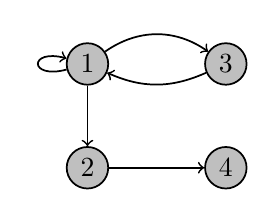
\begin{tikzpicture}
[every node/.style={inner sep=0pt}]
\node (1) [circle, minimum size=15.0pt, fill=lightgray, line width=0.625pt, draw=black] at (37.5pt, -25.0pt) {\textcolor{black}{1}};
\node (2) [circle, minimum size=15.0pt, fill=lightgray, line width=0.625pt, draw=black] at (37.5pt, -62.5pt) {\textcolor{black}{2}};
\node (3) [circle, minimum size=15.0pt, fill=lightgray, line width=0.625pt, draw=black] at (87.5pt, -25.0pt) {\textcolor{black}{3}};
\node (4) [circle, minimum size=15.0pt, fill=lightgray, line width=0.625pt, draw=black] at (87.5pt, -62.5pt) {\textcolor{black}{4}};
\draw [line width=0.625, ->, color=black, loop left] (1) to (1);
\draw [line width=0.625, ->, color=black] (1) to  [in=145, out=35] (3);
\draw [line width=0.625, ->, color=black] (3) to  [in=336, out=204] (1);
\draw [line width=0.625, ->, color=black] (1) to  (2);
\draw [line width=0.625, ->, color=black] (2) to  (4);
\end{tikzpicture}

\end{document}
